\section{Comparison}
Lastly, the performance of the baseline method and the final model was compared. For this comparison, both models were evaluated over 10 epochs. The results of this comparison are presented in Table \ref{tab: results}. This table visualizes the rewards obtained by each model, providing a clear depiction of their respective performances. The comparison underscores the significant improvement achieved by the final model over the baseline.


Figure \ref{fig: q-values} illustrates the predicted Q-values over a sequence of 150 frames, beginning from frame 50, to capture the game's dynamics during mid-game rather than at the start. Within this interval, Frame 19 exhibits the lowest Q-value, close to zero, indicating minimal expected future rewards. As shown in Figure \ref{fig: frame19}, corresponding to Frame 19, the ball is positioned on the right side of the screen, isolated from any nearby targets that could be struck in subsequent frames to accumulate points. This observation aligns with the low Q-value, reflecting the anticipation of limited future rewards.

Conversely, Frame 54 in Figure \ref{fig: frame54} shows the highest Q-value, suggesting substantial expected future rewards. Examining the corresponding Frame 54 in Figure z reveals the ball poised to hit a target, which would result in scoring points. This is corroborated by the significant increase in the current score to 1500, compared to the score of 100 in Frame 19. Additionally, the inversion of colors from black to white indicates a noteworthy event, in this case, the ball striking the target. These observations substantiate the high Q-value's implication of considerable future rewards, validating the model's predictive accuracy.
%Figure x shows the predicted Q-values over the time for 150 frames, starting from frame 50 that we have a look at the frames during mid game and not directly at the beginning. In this Zeitraum, Frame 19 has the lowest Q-value of nearly 0, that indicitates low future rewards. If we have a look at figure y, that represents the corresponding frame 19, we see the ball on the right of the screen without having any targets in the umgebung that he could hit in the next few frames to score some points, which confirms the hypothesis of low future rewards refelcting the low Q-value. On the other hand, frame 54 in the figure x has the highest q-value indicating high future rewards. Looking at the corresponding frame, displayed in figure z, we can see that the ball is in the moment to hit the target and gain some points. This hypothesis is also confirmed by the current score of 1500 that is much higher than the score of 100 in frame 19. Also the color invertion of black into white signalises, that something special has happened, in this case the ball hits at exactly this moment the target. These impressions confirm the hypothesis of high future rewards derived by the high q-value in figure x. 

\begin{figure}
    \centering
    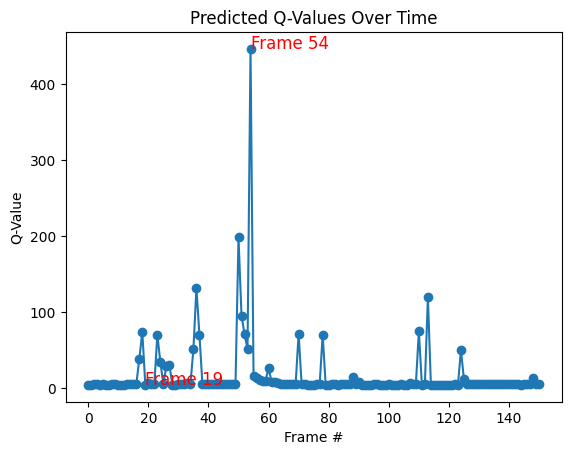
\includegraphics[width=0.8\linewidth]{graphics/q-values.png}
    \caption{The plot illustrates the predicted Q-values over a sequence of 150 frames, beginning from frame 50 and skipping the initial 50 frames to focus on the mid-game segment. The x-axis represents the frame number, while the y-axis shows the Q-value, indicating the expected future reward for the best action taken from that frame. The highest Q-value occurs at Frame 54, suggesting a significant positive event or reward, while the lowest Q-value is observed at Frame 19, potentially indicating a less favorable state or an immediate negative outcome. The significant fluctuations in Q-values highlight critical decision points and the agent's varying confidence levels throughout the game sequence, providing insights into the agent's decision-making process during mid-game play.}
    \label{fig: q-values}
\end{figure}

\begin{figure}
    \centering
    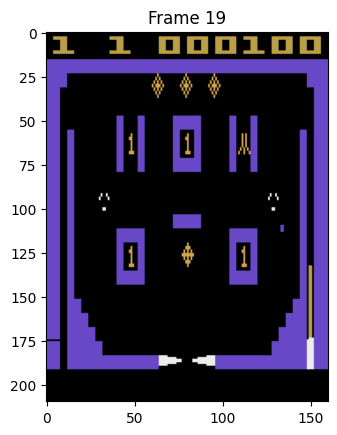
\includegraphics[width=0.7\linewidth]{graphics/frame19.png}
    \caption{The figure shows the 19th frame of the game. The ball is positioned on the right side of the screen, isolated from any nearby targets that could be struck in subsequent frames to accumulate points. This observation aligns with the low Q-value, reflecting the anticipation of limited future rewards.}
    \label{fig: frame19}
\end{figure}

\begin{figure}
    \centering
    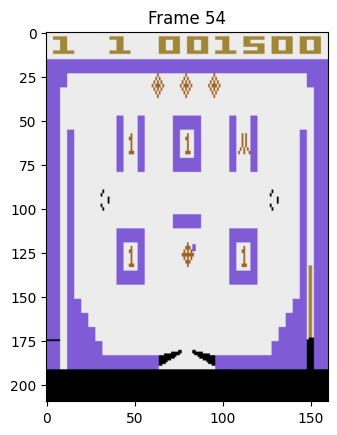
\includegraphics[width=0.7\linewidth]{graphics/frame54.png}
    \caption{Frame 54 shows the frame of the highest Q-value, suggesting substantial expected future rewards. The ball is poised to hit a target, which would result in scoring points. This is corroborated by the significant increase in the current score to 1500, compared to the score of 100 in Frame 19. Additionally, the inversion of colors from black to white indicates a noteworthy event, in this case, the ball striking the target. These observations substantiate the high Q-value's implication of considerable future rewards, validating the model's predictive accuracy.}
    \label{fig: frame54}
\end{figure}




\begin{table}[!h]
    \centering
    \begin{tabular}{lr}
        \toprule
         \textbf{Model} & \textbf{Average Reward per Epoch} 
         \\ \midrule
         Baseline & 2931.6  \\ \addlinespace
         DQN & 12078.8 \\ \addlinespace
         \bottomrule
    \end{tabular}
    \caption{Comparison of average rewards per epoch for baseline and DQN models in the Atari Video Pinball environment. The DQN model significantly outperforms the baseline model, achieving a substantially higher average reward per epoch. These models were compared over 5 epochs, which resulted in a total of 15 episodes.}
    \label{tab: results}
\end{table}
